\documentclass[convert={density=300,size=1080x800,outext=.png}]{standalone}
\usepackage{tikz}
\usepackage{tikz-network}
\begin{document}
	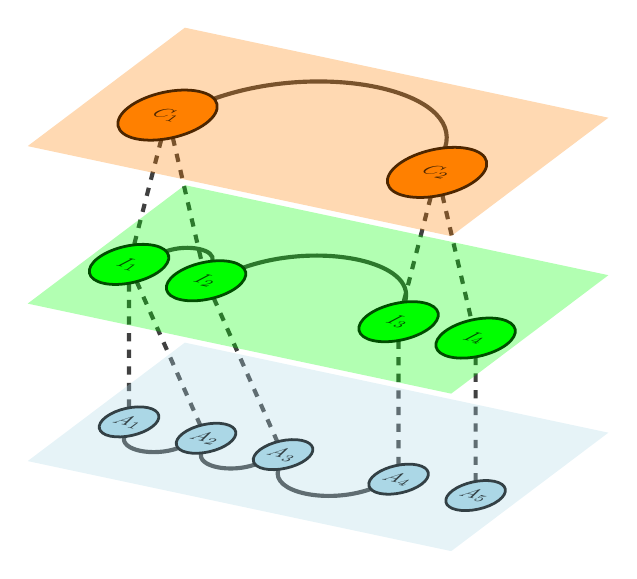
\begin{tikzpicture}[multilayer=3d]

\Vertex[x=1,label=$C_1$,layer=1, color = orange, size = 1]{A}
\Vertex[x=4.5,label=$C_2$,layer=1, color = orange, size = 1]{B}
\Vertex[x=0.5,label=$I_1$,layer=2, color = green, size = .8]{C}
\Vertex[x=1.5,label=$I_2$,layer=2, color = green, size = .8]{D}
\Vertex[x=4,label=$I_3$,layer=2, color = green, size = .8]{E}
\Vertex[x=5,label=$I_4$,layer=2, color = green, size = .8]{F}
\Vertex[x=0.5,label=$A_1$,layer=3, size = .6]{G}
\Vertex[x=1.5,label=$A_2$,layer=3, size = .6]{H}
\Vertex[x=2.5,label=$A_3$,layer=3, size = .6]{I}
\Vertex[x=4,label=$A_4$,layer=3, size = .6]{J}
\Vertex[x=5,label=$A_5$,layer=3, size = .6]{K}
\Edge[style=dashed](C)(G)
\Edge[style=dashed](C)(H)
\Edge[style=dashed](D)(I)
\Edge[style=dashed](A)(C)
\Edge[style=dashed](A)(D)
\Edge[style=dashed](B)(E)
\Edge[style=dashed](B)(F)
\Edge[style=dashed](E)(J)
\Edge[style=dashed](F)(K)

\Edge[bend=60](A)(B)
\Edge[bend=60](C)(D)
\Edge[bend=60](D)(E)
\Edge[bend=-60](G)(H)
\Edge[bend=-60](H)(I)
\Edge[bend=-60](I)(J)


\SetLayerDistance{-2}
\Plane[x=0,y=-1,width=5.5,height=2.5,color=orange,layer=1,NoBorder]
\Plane[x=0,y=-1,width=5.5,height=2.5,color=green,layer=2,NoBorder]
\Plane[x=0,y=-1,width=5.5,height=2.5, layer = 3,NoBorder]
\end{tikzpicture}
\end{document}
